\documentclass[12pt]{article}

\usepackage[a4paper, nomarginpar, total={170mm,257mm, left=25mm, right=15mm, top=20mm,bottom=20mm}]{geometry}
\pagestyle{plain}
\linespread{1.5}

\usepackage[italian,lithuanian]{babel}
\usepackage[utf8]{inputenc}
\usepackage{libertine}
\usepackage{graphicx}
\usepackage{floatflt}
\usepackage{blindtext}
\usepackage{enumitem}
\usepackage{amsthm}
\usepackage{subfig}
\usepackage{listings}
\usepackage{listingsutf8}
\usepackage{amsmath}
\usepackage{framed}
\usepackage{minibox}
\usepackage{float}
\usepackage{wrapfig}
\usepackage{longtable}
\usepackage[strict]{changepage}
\usepackage{pgfplots}
\usepackage{tikz}
\usetikzlibrary{matrix}
\pgfplotsset{width=11cm,compat=1.9}
\usepgfplotslibrary{external}
\tikzexternalize
\usepackage[L7x]{fontenc}


\usepackage{tgtermes}
\usepackage{indentfirst}

\usepackage{graphicx}
\usepackage{float}
\usepackage{caption}


\usepackage{hyperref}
\hypersetup{
colorlinks=true,
linkcolor=black,
filecolor=black,
urlcolor=blue,
citecolor=black
}

\usepackage{setspace}
\onehalfspacing
\usepackage[
backend=biber,
style=apa,
url=false,
sorting=nyt
]{biblatex}
\addbibresource{references.bib}

\begin{document}

\begin{titlepage}
\begin{figure}[t]
   \centering
\includegraphics[width=0.9\textwidth]{logo}
\end{figure}
\begin{center}
    \textsc{ \LARGE{Fundamentinių veiksmų įtaka Vilniaus Universiteto Studentų Investicinio fondo vertybinių popierių portfelio formavimui \\}}

	\vspace{30mm}
	\fontsize{7mm}{7mm}\selectfont 
    \textup{Vilniaus Universitetas}\\
\end{center}

\vspace{50mm}

\begin{minipage}[t]{1\textwidth}
	\flushright\textnormal{\large{\bf Paruošė:\\}}
	{\large Tautvydas Stasiulis}
\end{minipage}

\vspace{20mm}

\centering{\large{ 2019 m. birželio 17 d. }}

\end{titlepage}


\tableofcontents
\newpage
\section{Įvadas}

Net ir 2019 metais Lietuvoje finansinis raštingumas išlieka opi visuomenės problema. Finansinis raštingumas apima ne tik žinias apie finansus ar su finansais susijusias rizikas, tačiau ir šių žinių pritaikymą priimant veiksmingus sprendimus, kurie užtikrintų ne tik asmens, bet ir visos tautos finansinę gerovę. Lietuvos bankų asociacijos atlikto tyrimo rezultatai atskleidė, kad Lietuvoje net 22 proc. apklaustųjų neatsakė nė į vieną klausimą susijusį su pensijos planavimu, o 13 proc. neatsakė į klausimus apie investavimą. Esamą situaciją pablogino ir šiais metais įvykę pasikeitimai pensijų kaupimo sistemoje, kurie smarkiai sumažino šios sistemos patrauklumą. Bėgdami nuo netinkamai veikiančių pensijų fondų gyventojai pradėjo patys investuoti Baltijos regiono vertybinių popierių rinkoje, tačiau pradedantiems investuotojams tobulėti trukdo bazinių žinių stoka finansų sferoje. Sėkmingam investavimui yra būtina ne tik tam tikra filosofija ar asmeninė disciplina, bet ir kruopščiai atlikta fundamentinė vertybinių popierių analizė. Fundamentalioji analizė padeda suformuoti bendrą vaizdą apie įmonę, tačiau toks požiūris yra vienpusis, todėl sėkmingam vertybinių popierių atrankos procesui užtikrinti reikalinga fundamentinių ir techninių veiksnių įtakos vertybinių popierių portfelio formavimui įvertinimo sintezė. \cite{cibulskiene2006fundamentiniku}. Formuojant efektyvų vertybinių popierių portfelį kiekvienas racionalus investuotojas stengiasi pasiekti didžiausią pelningumą esant tam tikrai rizikai, arba mažiausią riziką esant tam tikram pelningumui. Pagrindinis rizikavimo tikslas, investuojant į akcijas, yra gauti didesnes pajamas, lyginant su alternatyviomis investicijomis. \cite{lileikiene2010akcijku}. Tirdamas hipotetinį VUSIF portfelį argumentuotai atsakysiu į išsikeltus klausimus:

\begin{itemize}
\item Ar įmonės esančios sudarytame portfelyje pateisina joms keliamus lūkesčius?
\item Kurias turimas pozicijas vertėtų parduoti? Kodėl? Kurias turimas pozicijas vertėtų didinti? Kodėl?
\end{itemize}


\section{Duomenų apžvalga}

\subsection{Taikyti metodai įmonių akcijos kursų grafikų tyrimui}
Duomenų šaltinis: \href{https://finance.yahoo.com/}{Yahoo finance}.

Duomenų pavadinimas: APG1L.VS., SAB1L.VS., TEL1L.VS., OLF1R.RG., VLP1L.VS., OMXBBGI.VS.

Alternatyvūs URL:
\begin{enumerate}
\item \href{https://finance.yahoo.com/quote/APG1L.VS?p=APG1L.VS&.tsrc=fin-srch}{Aprangos Group akcijos kurso duomenys}

\item\href{https://finance.yahoo.com/quote/SAB1L.VS?p=SAB1L.VS&.tsrc=fin-srch}{Šiaulių banko akcijos kurso duomenys}

\item\href{https://finance.yahoo.com/quote/TEL1L.VS?p=TEL1L.VS&.tsrc=fin-srch}{Telia akcijos kurso duomenys}

\item\href{https://finance.yahoo.com/quote/OLF1R.RG?p=OLF1R.RG&.tsrc=fin-srch}{Olainfarm akcijos kurso duomenys}

\item\href{https://finance.yahoo.com/quote/VLP1L.VS?p=VLP1L.VS}{Vilkyškių pieninės akcijos kurso duomenys}

\item\href{https://finance.yahoo.com/quote/\%5EOMXBBGI/}{Palyginamojo indekso duomenys}
\end{enumerate}

Duomenys reikalingi grafikų braižymui yra pateikiami .xts formatu. Duomenų atsisiuntimui naudojamas „quantmod“ funkcijų paketas ir funkcija getSymbols(). Reikalingų kompanijų akcijų kainas atsisiunčiame nurodytame periode iš „Yahoo Finance" puslapio. Braižydami grafikus .xts formatu galima pritaikyti techninės analizės indikatorius, kurie yra integruoti į candlechart() ir chart\_Series() funkcijas. Turimi akcijų kursų duomenys yra apjungti į vieną .xts formato lentelę ir vieną „dataframe" tipo duomenų lentelę. Xts tipo lentelė yra naudojama techninei portfelį sudarančių įmonių analizei. „Dataframe" tipo lentelėje yra sudaromas hipotetinis investicinis portfelis, kuris remiasi Vilniaus Universiteto Studentų Investicinio fondo portfeliu. Hipotetinis portfelis yra sudaromas sudauginant turimų akcijų kiekį su atitinkamos dienos akcijų kaina. Reikia paminėti, jog istoriniai akcijos kurso duomenys neatsižvelgia į infliacijos rodiklį, todėl nėra taikomas diskontavimo metodas. Fundamentalioji analizė yra vienas pagrindinių metodų, padedančių įvertinti akcijos vertę, analizuojant pagrindinius įmonės kapitalo rinkos rodiklius. Iš esmės tai reiškia, kad fundamentalioji analizė apima tik tuos rodiklius, kurie susiję su pačia įmone, t. y. pardavimų pajamos, dividendai, pelnas ir t.t., ir nenagrinėja pačios kapitalo rinkos būklės. Remiantis fundamentaliąja analize nagrinėjama įmonės veikla siekiant nustatyti, ar tuo momentu
įmonių akcijas reikia parduoti ar pirkti. \cite{cibulskiene2006fundamentiniku}
Apskaičiavus portfelio ir palyginamojo indekso vieneto vertes yra nubraižomas palyginamasis grafikas. Jeigu portfelis aplenks indeksą, tai portfelis sudarytas sėkmingai, jeigu ne, tai portfelį reiktų optimizuoti ir keisti investavimo strategiją ar turimas pozicijas. Mokslinėje literatūroje išskiriamos dvi pagrindinės vertybinių popierių portfelio valdymo strategijos: pasyvus valdymas ir aktyvus valdymas. Pasyvi valdymo strategija kitaip dar vadinama „pirk ir laikyk“ investavimo strategija nereiškia, kad investuotojas nieko nedaro. Jis turi stebėti savo vertybinių popierių portfelį, kad jis atitiktų jo tikslus ir leidžiamas rizikos ribas, nes sąlygos finansiniame sektoriuje greitai kinta. \cite{lileikiene2010akcijku}. Darome prielaidą, kad investicinis portfelis yra valdomas pasyviai t.y. portfelio valdytojas nespekuliuoja vertybinių popierių biržoje su turimomis pozicijomis.


\subsection{Taikyti metodai įmonių finansinių rodiklių analizei}

Alternatyvūs URL:

\href{https://www.nasdaqbaltic.com/market/?pg=reports&lang=lt}{Baltijos biržoje kotiruojamų įmonių finansinės ataskaitos}

Puslapyje pateiktos įmonių ketvirčių ir konsoliduotos metinės finansinės ataskaitos, kurios reikalingos fundamentinei analizei atlikti. Finansines ataskaitas buvo galima atsisiųsti ir per „YahooFinance“, tačiau 2018 metų spalio mėnesį ši galimybė buvo panaikinta. Deja, bet finansinius rodiklius teks išrinkti rankiniu būdu. Iš išrinktų duomenų yra paskaičiuojamas fundamentinei analizei reikalingi rodikliai : P/E, P/B, gryno pelno pokyčius, EPS, EBITDA pokyčiai.
\newpage
\section{Rezultatai}
Fundamentalios analizės metodu buvo nagrinėjamos penkios įmonės, kurios ne tik patenka į Vilniaus Universiteto Studentų Investicinio fondo portfelį, bet ir yra kotiruojamos Baltijos šalių vertybinių popierių biržoje. Fundamentinė analizė atliekama 3 etapais. Pirmiausia yra tiriami makroekonominiai rodikliai, po to sektoriaus rodikliai ir pereinama prie įmonės rodiklių. Pagrindinis šios analizės privalumas yra tas, jog yra įvertinama daug kintamųjų, kurie įtakoja pasirinktus vertybinius popierius, todėl turimas platus informacijos spektras sprendimui priimti. \cite{klavcok2018fundamentines}. Techninės analizės bei fundamentinės analizės tyrimo objektai skiriasi, kadangi fundamentinė analizė tiria rodiklius už vertybinių popierių rinkos, o techninė – pačią vertybinių popierių rinką. \cite{klavcok2018fundamentines}.Aktyvių strategijų šalininkai stengiasi pasiekti geresnių rezultatų negu rinkos vidurkiai. Šie investicijų valdytojai aktyviai naudojasi naujausia analitine informacija, sudėtingesnėmis investavimo priemonėmis (pvz., išvestinėmis) ir yra aktyvesni, keičiant vieną turtą į kitą. \cite{kalinauskas2003investicijku}. Atlikus tiek fundamentinę, tiek ir techninę analizę galima matyti, jog net keturios iš penkių įmonių atsilieka nuo palyginamojo indekso, todėl galime drąsiai teigti, jog hipotetinis investicinis portfelis yra sudarytas netinkamai. Situacija gelbėja tik tai, jog investicinis portfelis yra ganėtinai diversifikuotas, todėl yra sumažinama rizika akcijų kainų kritimo atveju. Tyrimo metu daroma prielaida, jog portfelis yra valdomas pasyviai.

\subsection{Apranga Group apžvalga}
Blogiausias pirkinys portfelyje yra „Apranga group“ akcijos, kurios nuo 2016 m. krito beveik 22 proc. Šiais metais įmonė planuoja papildomai investuoti apie 10-15 mln. eurų į turimų parduotuvių renovaciją ir plėtrą, pernai buvo skirta kiek daugiau negu 6 mln. eurų. 2018 metais investuotojai smarkiai nuvertino „Aprangos" akcijas dėl suprastėjusių finansinių rezultatų ir „Aprangos" akcininkų dalyvavimo „MG BALTIC" skandale. Blogi  „Aprangos Group" rodikliai rodo, kad įmonė nesusitvarko su turimu turtu, tačiau Altman'o modelio pritaikymas užtikrino, jog bankroto tikimybė yra maža. Vienas pirmųjų autorių, panaudojusių daugiamatę diskriminantinę analizę bankrotui prognozuoti, yra Edward I. Altman. 1968 m. \cite{dzikevivcius2015finansiniku}. Nors „Aprangos“ pardavimai ir išmokamų dividendų kiekis augo nuo pat 2015 m., tačiau ženkliai sumažėjusi EBITDA ir pralaimima kova tiesioginiams konkurentams („H\&M”) verčia nerimauti šios įmonės ateitimi.


\begin{figure}[H]
\captionsetup{justification=centering}
\center
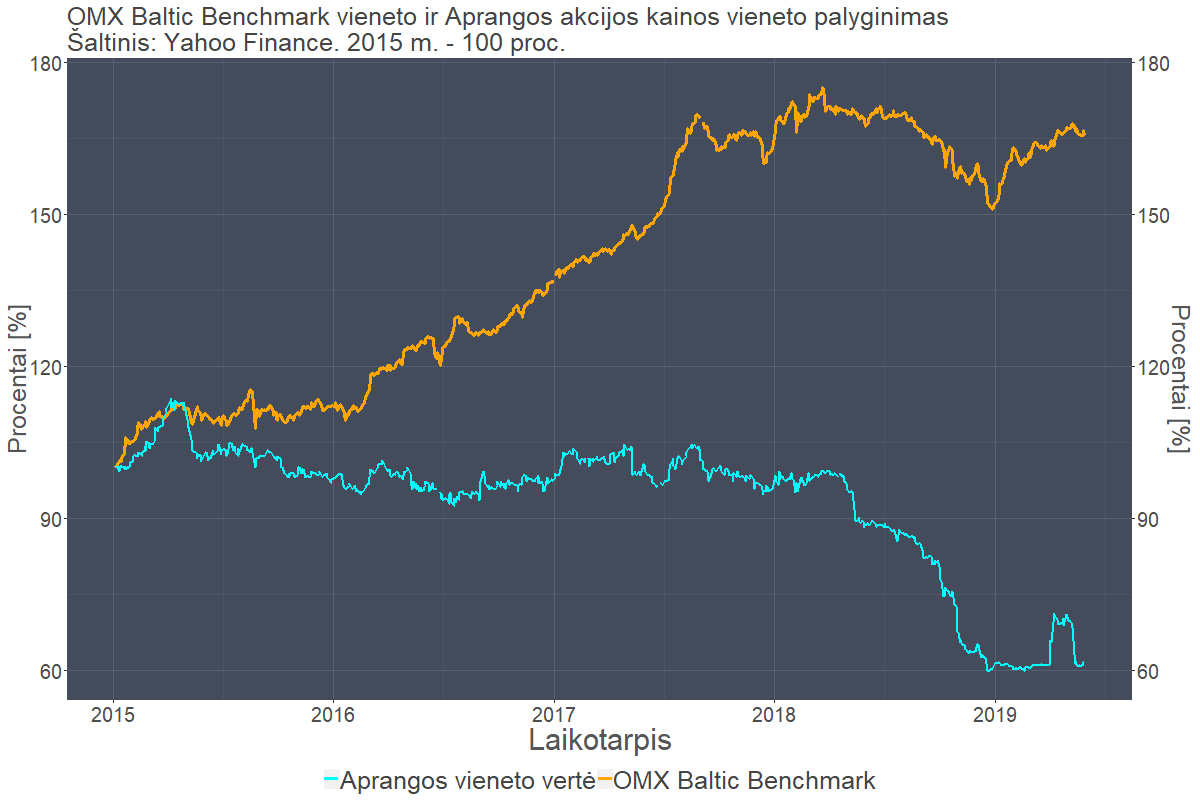
\includegraphics[scale=0.4]{APG.png}
\caption{OMX Baltic Benchmark vieneto ir Aprangos akcijos kainos vieneto palyginimas \newline
Šaltinis: Sudaryta autoriaus}
\end{figure}
\subsection{Olainfarm apžvalga}
Kita smarkiai nuvylusi įmonė yra Latvijos farmacijos milžinė „Olainfarm“. Šios įmonės veiklą galime suskirstyti į du etapus: pirmasis etapas baigėsi sulig pagrindinio akcininko ir įmonės vadovo Valerijaus Maligino mirtimi, o antrasis etapas tęsiasi iki šios dienos, ši tendenciją puikiai atsispindi ir akcijos kainos grafike. Mirus įmonės vadovui kompanijos vadovybė nesugebėjo pasidalinti valdžios ir palikto turto, todėl vidiniai nesutarimai suskaldė įmonės galimybę tinkamai veikti. Atlikus fundamentinę analizę galima matyti, jog įmonės akcijos šiuo metu yra smarkiai nuvertinamos, P/E rodiklis siekia vos 11,83, nors sektoriaus vidurkis svyruoja apie 35,5. Jeigu „Olainfarm“ sugebės susitvarkyti su vidinėmis problemomis, tai labai tikėtina, jog sugebės susigrąžinti prarastą investuotojų pasitikėjimą.

\begin{figure}[H]
\captionsetup{justification=centering}
\center
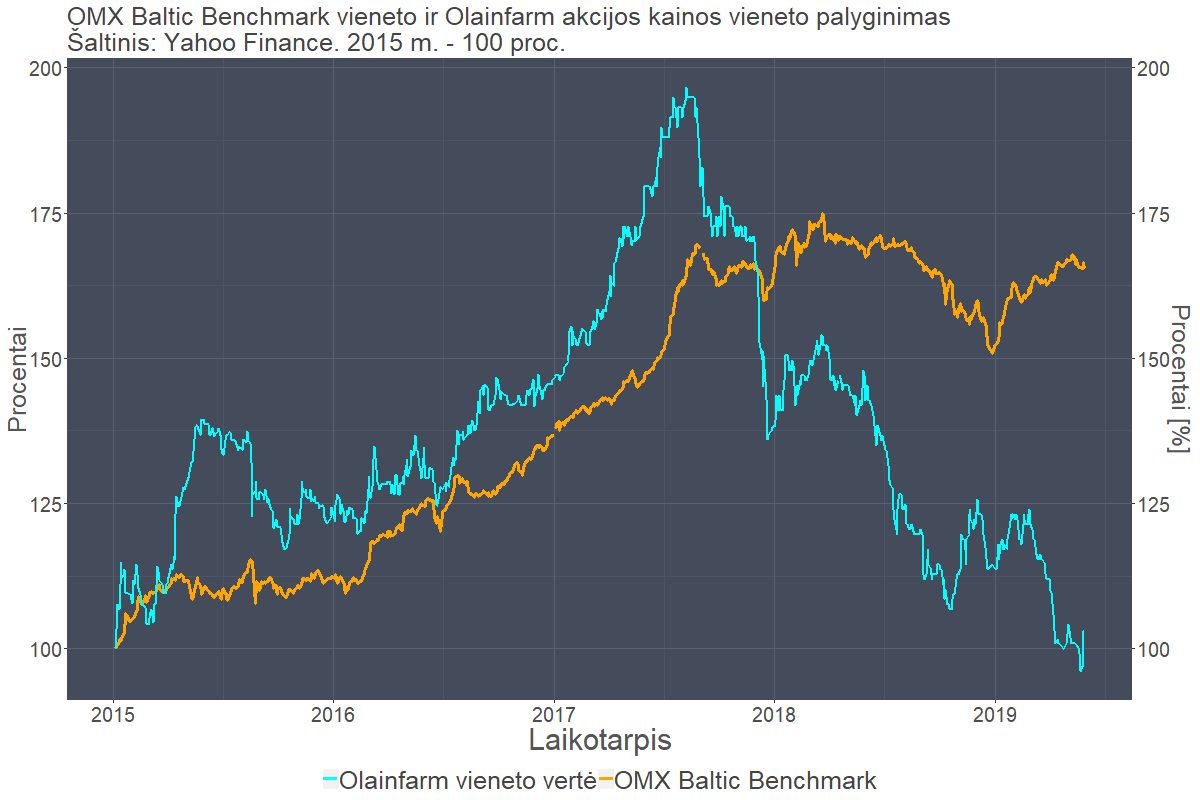
\includegraphics[scale=0.4]{OLF.png}
\caption{OMX Baltic Benchmark vieneto ir Olainfarm akcijos kainos vieneto palyginimas \newline
Šaltinis: Sudaryta autoriaus}
\end{figure}

\subsection{Vilkyškių pieninės apžvalga}
Viena didžiausių Lietuvoje pieno perdirbimo įmonių pirmąjį šių metų ketvirtį patyrė beveik 0,82 mln. eurų konsoliduoto grynojo pelno nuostolį. Nors nuo 2018 metų balandžio mėnesio pieno supirkimo kaina stambiesiems ūkiniams padidėjo 8,4 proc., tačiau ženkliai išaugę pardavimo kaštai suvalgė visas iki tol uždirbtas pajamas. Uždirbtų pajamų net neužteko padengti administracinėms ir logistikos sąnaudoms. Kruopščiai išnagrinėjus konsoliduotą „Vilkyškių Pieninės“ metinę ataskaitą galima pamatyti, jog didžiąją dalį sąnaudų sudarė techninės įrangos ir nekilnojamo turto nusidevėjimas. Padidėjusį nekilnojamo turto nusidevėjimą paaiškina naujas „Vilkyškių pieninės“ projektas į kurį buvo investuota kiek daugiau negu 30 mln. eurų per 3 metų laikotarpį. Šis projektas, tai neseniai pastatyta išrūgų perdirbimo gamykla Tauragėje, kuri iki šiol dirbo bandomuoju režimu. Žvelgiant į įmonės potencialą ilguoju laikotarpiu, reiktų atkreipti dėmesį į Estijos pienininkus. Pieno gamintojų kooperatyvo „E-piim“ planuose grandiozinio dydžio projektas – pieno perdirbimo gamykla galinti perdirbti iki 1000 tonų žaliavinio pieno per dieną. Jeigu Estijos pienininkų užmojis bus įgyvendintas, tai nuo 2021 m. Baltijos regionas turės dar vieną stiprų žaidėją pieno rinkoje. Prie nerimą keliančių ir potencialius investuotojus atbaidančių veiksnių galima pridėti ir korupcijos skandalą „Vilkyškių Pieninės“ viduje. Vienam įmonės valdybos nariui skirta 200 tūkst. eurų bauda už viešai investuotojams neatskleistos informacijos panaudojimą siekant asmeninės naudos. Nepasitvirtino ir rinkos analitikų prognozės, kurie tikėjosi didesnio įmonių pelningumo pirmąjį šių metų ketvirtį dėl padidėjusio eksporto. Didelę grėsmę Europos pieno rinkai kelią ir galimas „hard - Brexit“ scenarijus, kuris galėtų rimtai apsunkinti pieno produktų prekybos su Didžiąja Britanija procesą ir taip galutinai pasiųsti „Vilkyškių Pieninę“ į techininį nokautą.

\begin{figure}[H]
\captionsetup{justification=centering}
\center
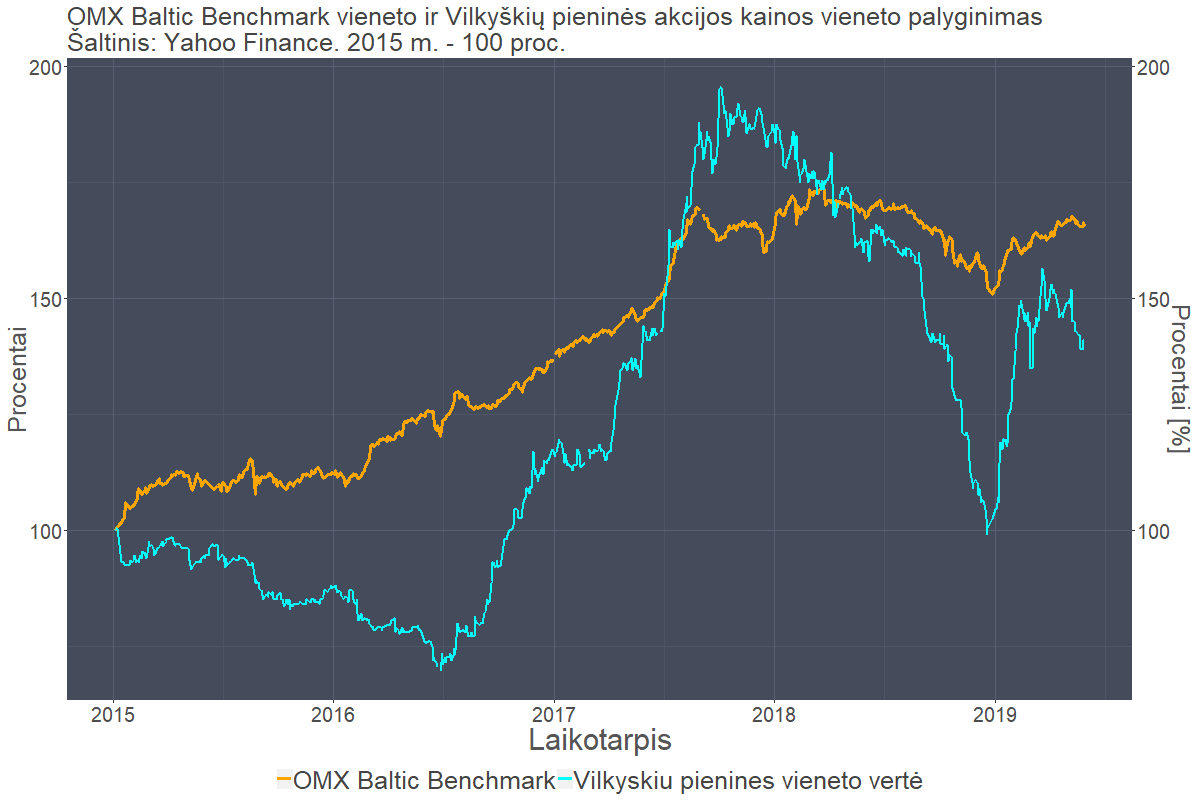
\includegraphics[scale=0.4]{VLP.png}
\caption{OMX Baltic Benchmark vieneto ir Vilkyškių pieninės akcijos kainos vieneto kainos palyginimas \newline
Šaltinis: Sudaryta autoriaus}
\end{figure}

\subsection{Šiaulių banko apžvalga}

Stulbinančius rezultatus rodantis „Šiaulių Bankas“ yra geriausias ir kol kas vienintelis sudaryto portfelio pirkinys, kuris stabiliai lenkia palyginamąjį „OMX Baltic Benchmark“ indeksą nuo pat 2015 m. ir neša beveik 350 proc. siekiančią grąžą. 2018 metai bankui buvo itin sėkmingi – 12 proc. išaugo gyventojams suteiktų indėlių skaičius ir 8 proc. padidėjo išduotų paskolų kiekis. Metinis grynasis pelnas siekęs 53 mln. eurų 2018 m. padidėjo net 64 proc. lyginant su 2017 m. metiniais rodmenimis. Vasario mėnesio pradžioje „Šiaulių Banko“ atstovai išplatino pranešimą, kuriame teigiama, jog bankas gavo Vokietijos federalinės priežiūros institucijos leidimą teikti paslaugas Vokietijoje. Atstovų teigimu, bankas iš pradžių teiks tik terminuotų indėlių paslaugas, tačiau ateities planuose numatoma suteikiamų paslaugų diversifikacija ir plėtimąsis į kitas Europos Sąjungos šalis. Įsitvirtinti Vokietijos rinkoje gali būti sudėtingas uždavinys, tačiau sėkmingai įveikti vietiniai konkurentai reikštų, jog didžiulė Vokietijos rinka taptu tramplinu į naujas aukštumas. Banko akcininkai nesitiki staigaus plėtimosi, tačiau geografinis indėlių išskaidymas padėtų sumažinti riziką, masinio indėlių atsiėmimo atveju. Panagrinėjus „Šiaulių Banko“ finansines ataskaitas galima pamatyti, jog akcijos kainos ir nuosavybės santykis, dar žinomas kaip (angl. Price/Book), siekia vos 1,05, o kainos ir pelno santykis (angl. Price/Earnings) – 6,5. Net „Danske bank“, kurio akcijos kaina krito beveik per pusę (dėl pinigų plovimo skandalo) P/E rodiklis yra aukštesnis negu „Šiaulių Banko“ ir siekia 8. 

\begin{figure}[H]
\captionsetup{justification=centering}
\center
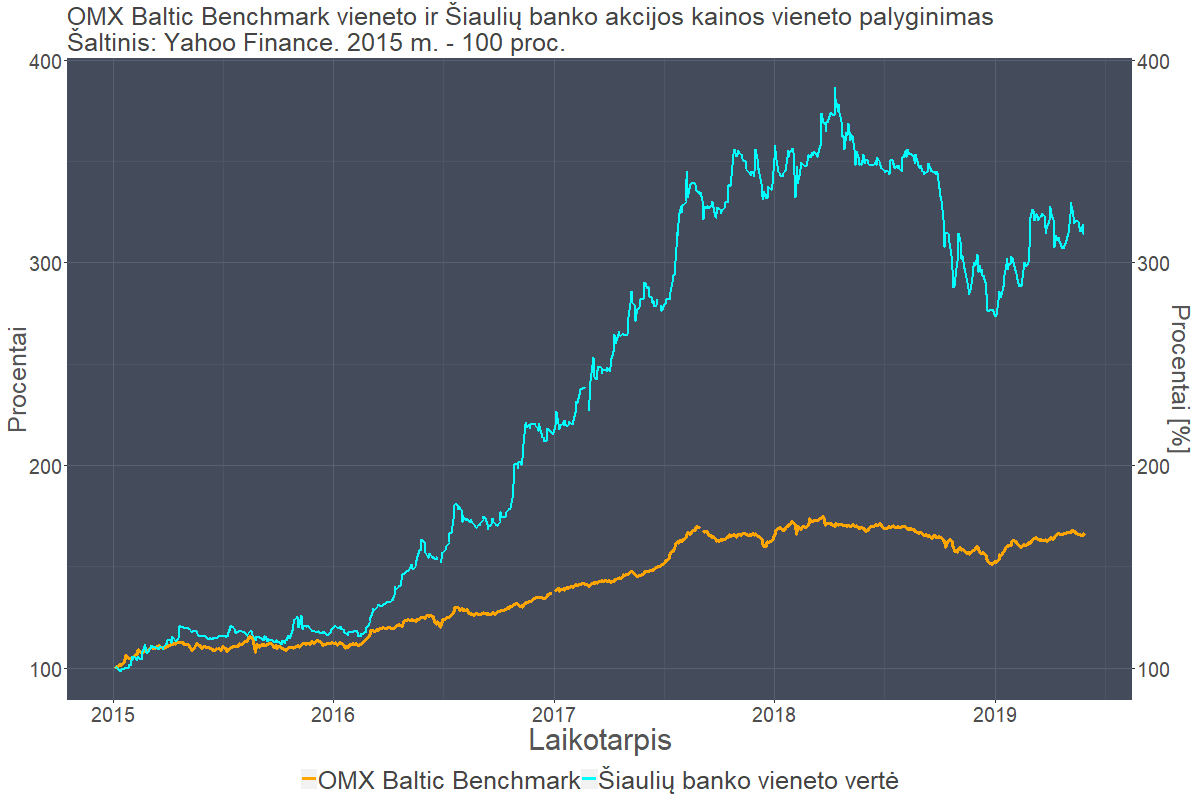
\includegraphics[scale=0.4]{SAB.png}
\caption{OMX Baltic Benchmark vieneto ir Šiaulių banko akcijos kainos vieneto palyginimas \newline
Šaltinis: Sudaryta autoriaus}
\end{figure}

\subsection{Telia apžvalga}
Praėję metai telekomunikacijų milžinei „Telia Lietuva“ buvo ganėtinai sėkmingi. Per visus 2018 – uosiuos metus „Telia“ uždirbo net 9 proc. didesnę EBIT lyginant su praeitų metų rezultatais.  Jeigu padalintume visą uždirbtą pelną prieš apmokestinimą iš vertybinių popierių biržoje kotiruojamų „Telia“ akcijų kiekio, tai gautume, kad vienai akcijai tenka apie 9,5 cento pelno. Taip pat svarbu paminėti, jog per visus 2018 m. labiausiai augo išmaniosios televizijos vartotojų kiekis, kuris padidėjo beveik 10 proc. lygintant su 2017 metų duomenimis. Nors EBIT ir augo, tačiau laisvųjų pinigų srautas (angl. free cash flow) smuko ir sudarė tik 46,7 mln. eurų. Laisvų pinigų srauto rodiklis parodo, kiek realių pinigų lieka įmonei iš pagrindinės įmonės veiklos ir kiek uždirbtų pinigų įmonė yra pajėgi grąžinti savo akcininkams. Šiais metais „Telia“ nusprendė nekeisti išmokamų dividendų politikos ir per kasmetinį akcininkų suvažiavimą paskelbė, kad dividendais bus išmokėta 80 proc. įmonės pelno. Akcininkus taip pat pradžiugino žinia, jog įmonė ketina efektyvinti įmonės veiklos struktūrą. Veiklos efektyvinimo plane nurodoma, jog įmonė ketina atleisti dalį darbuotojų, o likusią dalį perkelti į dukterinė įmonę - „Telia Global Service Lithuania“. Žvelgiant į įmonės potencialą ilguoju laikotarpiu ir esančią finansinę padėtį galima teigti, jog smarkaus akcijos kurso pakilimo neišvysime, tačiau smarkesnį vėjo gūsį gali atnešti nauja „Telia" paslauga - „5G“ internetas.
\begin{figure}[H]
\captionsetup{justification=centering}
\center
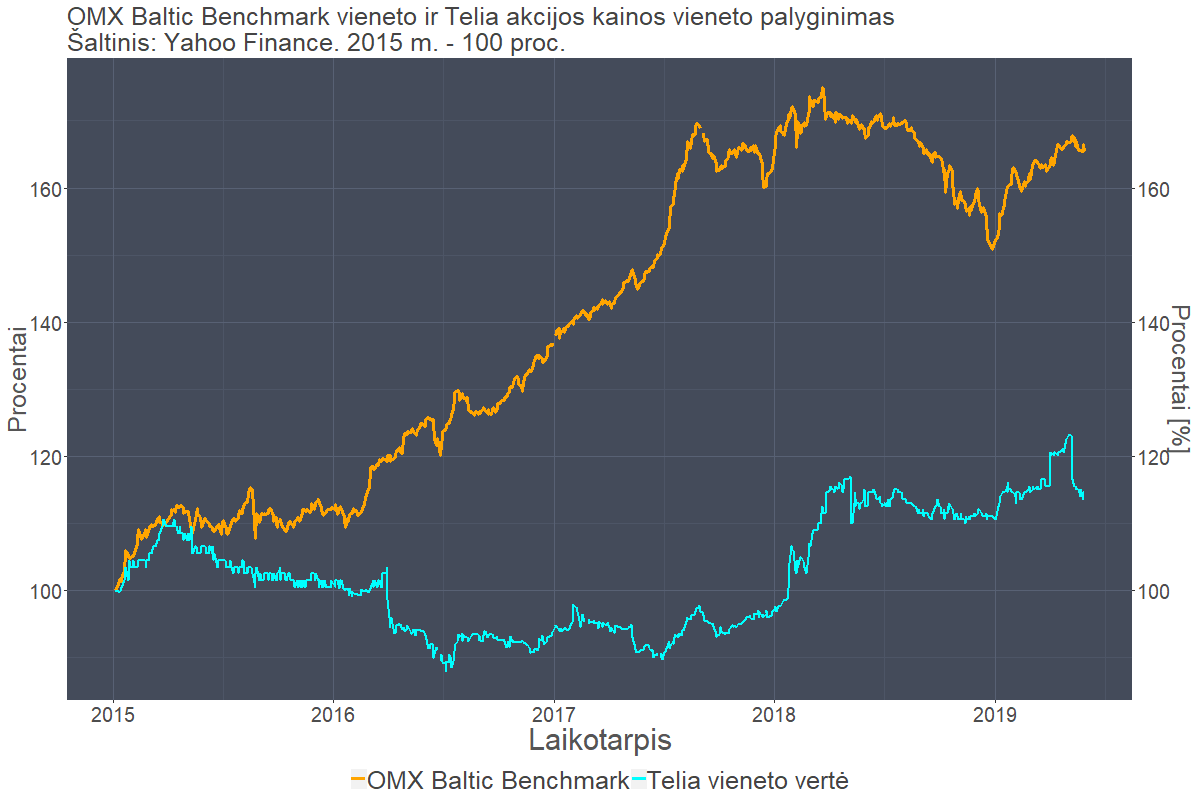
\includegraphics[scale=0.4]{TEL.png}
\caption{OMX Baltic Benchmark vieneto ir Telia akcijos kainos vieneto palyginimas \newline
Šaltinis: Sudaryta autoriaus}
\end{figure}

\section{Išvados}

Iš pateikto grafiko lengva pamatyti, jog procentinis skirtumas tarp palyginamojo „OMX Baltic Benchmark" vieneto vertės ir hipotetinio portfelio vieneto vertės yra ganėtinai didelis - siekia beveik 50 proc. Reiktų atsižvelgti į tai, kad hipotetinis investicinis portfelis buvo valdomas pasyviai, todėl portfelio valdytojas nesiimdavo veiksmų, jeigu rinkoje pasikeisdavo situacija. Net keturios portfelį sudariusios įmonės nepateisino joms keliamų lūkesčių, tiek  „Olainfarm", tiek ir „Vilkyškių pieninė" rodė neblogus rezultatus, tačiau pastovūs skandalai ir netinkamas vadovavimas trukdo sėkmingai tęsti veiklą. Sėkmingiausias portfelio pirkinys -  „Šiaulių banko" akcijos, kurių vertė išaugo beveik 3,5 karto nuo 2015 m.
Įvertinus atliktą fundamentinę analizę galima teigti, kad portfelį vertėtų sudaryti iš naujo ieškant geresnių pirkinių Baltijos regiono vertybinių popierių biržoje. Galima pasidžiaugti tik tuo, kad per 4 metų periodą hipotetinis investicinis portfelis atnešė 20 proc. siekiančią  „popierinę" grąžą (dar tolokai iki 10 proc. grąžos per metus). Kita vertus, jeigu investuotas būtų investavęs į palyginimąjį indeksą, būtų uždirbęs kiek daugiau negu 65 proc. siekiančią grąžą per 4 metų periodą.

Ko iš to galima pasimokyti? Vertybinių popierių rinka jautriai reaguoja į pasirodančias naujienas. Reikia nepamiršti, kad pirmieji, kurie reaguoja į įvykius dažniausiai būna spekuliantai, kurie akcijas laiko tik kelias dienas ir stengiasi išlošti iš akcijos kainos pokyčio. Jeigu apie įmonę pasirodo bloga žinia, tai dar nereiškia, kad viskas prarasta - kainai pasikoregavus galima surasti stiprų paramos lygį, kuris taps puikiu pirkiniu „long" tipo pozicijai. Nors Baltijos regiono biržai trūksta likvidumo, tačiau net ir čia galima prarasti dideles pinigų sumas. Pradedančiajam investuotojui yra ganėtinai sunku aplenkti palyginamąjį indeksą, tačiau tinkamai parinkta strategija, rizikos valdymas, disciplina ir savalaikiai sprendimai padės susikurti finansinę nepriklausomybę.

\begin{figure}[H]
\captionsetup{justification=centering}
\center
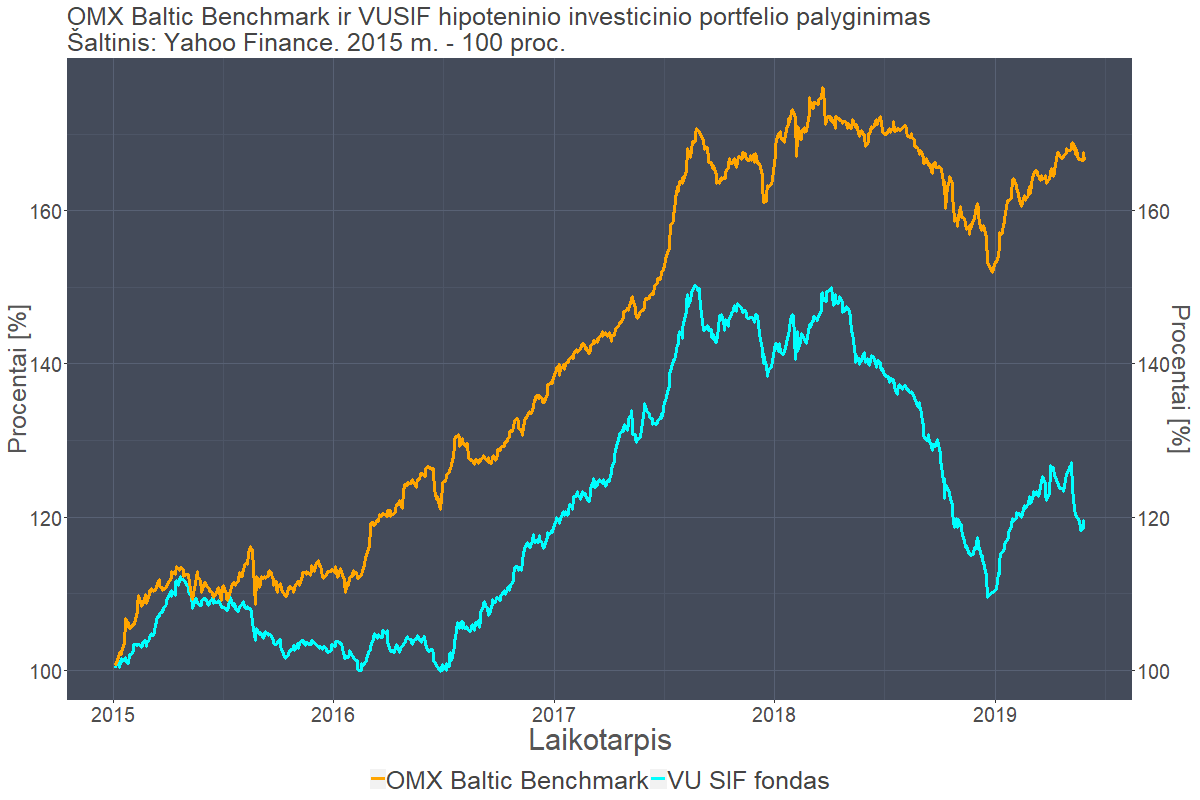
\includegraphics[scale=0.4]{PORTFELIS.png}
\caption{OMX Baltic Benchmark vieneto ir VUSIF hipoteninio portfelio vieneto kainos procentinis pokytis \newline
Šaltinis: Sudaryta autoriaus}
\end{figure}
\section{Priedai}
\begin{table}[H]
\captionsetup{justification=centering}
\centering
\begin{tabular}{l|c|c|l|}
\cline{2-4}
 & \textit{\textbf{Rodiklis}}             & \textit{\textbf{Tūkst. eurų}} & \textbf{} \\ \cline{2-4} 
 & \textbf{Trumpalaikis turtas}           & \textit{810}                  & tūkst.    \\ \cline{2-4} 
 & \textbf{Trumpalaikiai įsipareigojimai} & \textit{300}                  & tūkst.    \\ \cline{2-4} 
 & \textbf{Turtas}                        & \textit{65351}                & tūkst.    \\ \cline{2-4} 
 & \textbf{Nepaskirstytas pelnas}          & \textit{1094}                 & tūkst.    \\ \cline{2-4} 
 & \textbf{EBIT}                          & \textit{15563}                & tūkst.    \\ \cline{2-4} 
 & \textbf{Kapitalizacija}                & \textit{88000}                & tūkst.    \\ \cline{2-4} 
 & \textbf{Pardavimų pajamos}             & \textit{187207}               & tūkst.    \\ \cline{2-4} 
 & \textbf{Įsipareigojimai}               & \textit{12275}                & tūkst.    \\ \cline{2-4} 
\end{tabular}
\caption{Aprangos Group 2018 m. konsoliduotos finansinės ataskaitos rodikliai \newline
Šaltinis: Sudaryta autoriaus. Duomenys paimti iš Nasdaq Baltic}
\end{table}

Altmano modelio formulė:
\begin{equation}
Z = 0.012 · X_1 + 0.014 · X_2 + 0.033 · X_3 + 0.006 · X_4 + 0.999 · X_5
\end{equation}

\begin{equation}
X_1 = \frac{Turtas}{Apyvartinis \ kapitalas \ }
\end{equation}

\begin{equation}
X_2 = \frac{Turtas}{Nepaskirstytas \ pelnas \ }
\end{equation}

\begin{equation}
X_3 = \frac{Turtas}{Pelnas \ iki \ apmokestinimo \ }
\end{equation}

\begin{equation}
X_4 = \frac{ Įsipareigojimai}{Akcinio \ kapitalo \ rinkos \ vertė \ }
\end{equation}

\begin{equation}
X_5 = \frac{Turtas}{Pardavimo \ pajamos \ }
\end{equation}

\begin{quote}
\center
Altmano modelio pritaikymas „Aprangos Group" įmonei
\end{quote}

\begin{equation}
Z =2.912975
\end{equation}

\begin{table}[H]
\captionsetup{justification=centering}
\centering
\begin{tabular}{|c|c|}
\hline
\textbf{Rodiklis} & \textbf{Reikšmė} \\ \hline
\textbf{X1}       & 0.007804012      \\ \hline
\textbf{X2}       & 0.01674037       \\ \hline
\textbf{X3}       & 0.2381448        \\ \hline
\textbf{X4}       & 7.169043         \\ \hline
\textbf{X5}       & 2.864639         \\ \hline
\end{tabular}
\caption{Altmano modelio rodikliai.
Šaltinis: Sudaryta autoriaus}
\end{table}
\newpage
\section{Literatūros sąrašas}

\nocite{*}
\printbibliography[title={Naudota literatūra}]

\end{document}